% !TeX root = root.tex
% !TeX spellcheck = en_US
\section{GAP-exercise}
\subsection*{a)}
To compute the number of primitive permutation groups up to permutational equivalence, we use the GAP function \textit{NrPrimitiveGroups}. 

\lstinputlisting[language=gap]{ex5a.g}

Then for degrees $d = \{1,\dots, 100\}$ we get

\hspace*{-1cm}
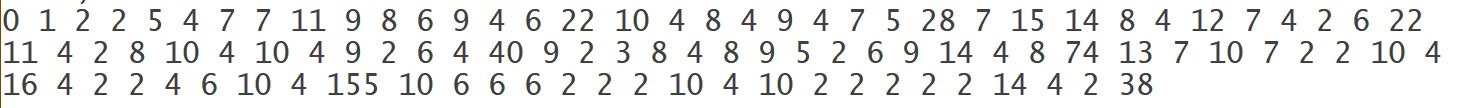
\includegraphics[width=17cm]{ex5}

\subsection*{b)}
We determine the possible number of minimal normal subgroups of primitive permutation groups of degree $d = \{1,\dots, 50\}$ as follows:

\lstinputlisting[language=gap]{ex5b.g}

We obtain that all groups except the trivial group have exactly one minimal normal subgroup.

\subsection*{c)}
Based on the results from b) we state the conjecture that primitive permutation groups except the trivial group have a unique minimal normal subgroup.